% !TEX TS-program = pdflatexmk
% !BIB TS-program = bibtex

\documentclass[12pt, a4paper, twoside]{book}
\usepackage{import}
\subimport{../}{preamble}
\ExecuteBibliographyOptions{articletitle=false}
\standalonetrue
\onehalfspacing
\begin{document}

\begin{singlespace}
{\color{white}
\chapter{Plasmon Interactions in Tip Dimers}}
\end{singlespace}

\AddToShipoutPictureBG*{ \AtPageUpperLeft{ \put(0,-240)
{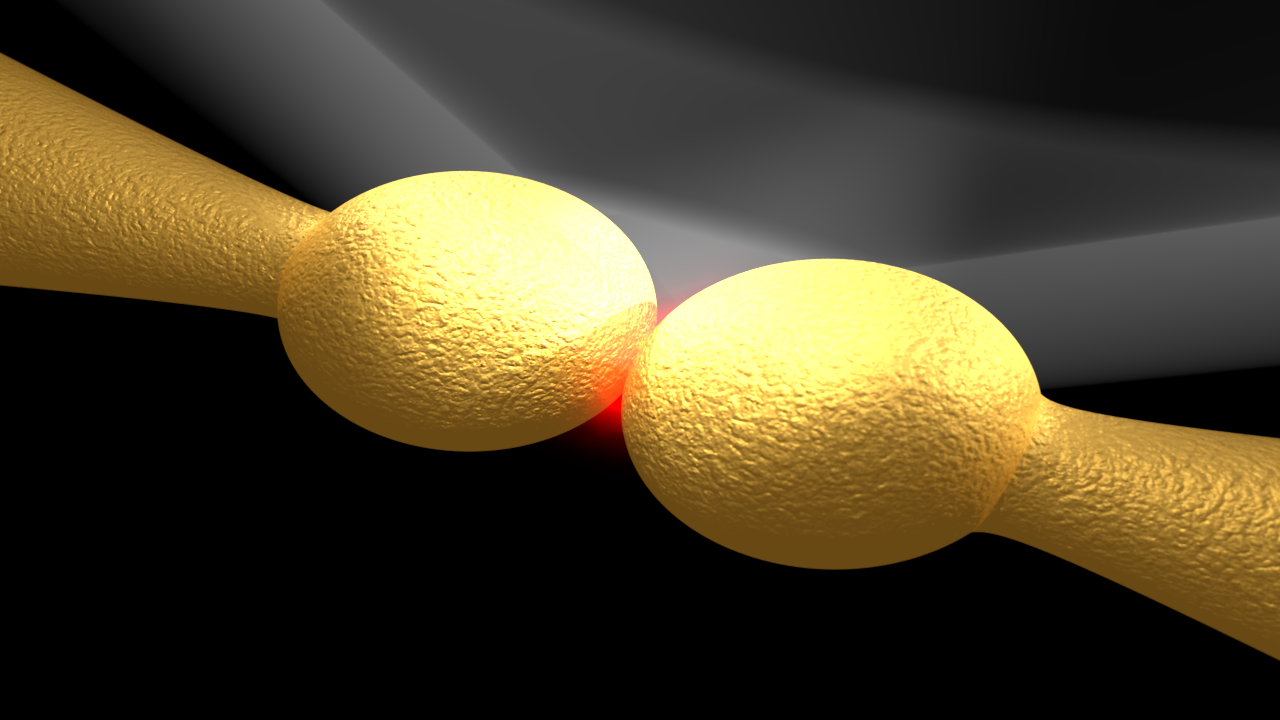
\includegraphics[width=\paperwidth, clip=true, trim=0 80 0 100]{figures/chapter_cover.png}}
}}

Plasmons that are experimentally identifiable as optical scattering resonances are generally structurally tuneable and exhibit coupling with other plasmons. Tunability therefore becomes a characteristic test to identify if a specific resonance is indeed due to plasmon excitation. With respect to tips, coupling between two tips can be used to determine whether observed resonances behave plasmonically.
Furthermore, since it is the coupling between plasmons that causes the large, exploitable field enhancements, it is important to understand how this effect occurs with tip structures. To fully characterise a plasmonic tip for application in processes such as TERS it's coupling must be known and understood.

Coupling between different tip morphologies is dynamically studied to demonstrate the plasmonic capabilities. Tips are generally coupled with another tip to maximise the optical accessibility of the gap. For two spherical tips the result is a structure which, in some sense, mimics a AuNP dimer. Taking advantange of this similarity allows fundamental plasmonics to be explored using a dynamic dimer system.

%\subimport{./}{quantum_effects}
\subimport{./}{tip_dimer_interactions}

\section{Conclusions}

Multiple different combinations of tips in a dimer configuration are used to probe plasmon coupling. Sharp Au tips exhibit no obvious plasmon resonances under far-field illumination and no gap mode coupling is observed with other sharp Au tips or spherical Au tips. This is caused by the lack of antenna modes in the sharp tip geometry.
Plasmons excited at the apex of spherical Au tips, on the other hand, interact and couple to form bonding hybridised modes. The behaviour of these modes is as expected, with similarity to plasmons in AuNP dimers. The inherent asymmetry between the large spherical tip structures leads to a more complex scattering result wherein anti-bonding modes are no longer dark. Their evolution into gap modes is something not previously seen before.

By using such dimer structures the influence of quantum effects, specifically quantum tunnelling, can be probed for sub-nm gaps. The irreproducibility between

\ifstandalone
\begin{singlespace}
\fontsize{8pt}{1em}\selectfont
\printbibliography[notcategory=fullcited]
\end{singlespace}
\fi

\end{document}